\section{Meanshift和Camshift}

\begin{frame}
    \frametitle{Meanshift背后的数学思想}
    Meanshift在统计学中是一种聚类(clustering)方法

    Meanshift在目标跟踪上的的核心思想是,让目标和采样区域的颜色、纹理等特征尽量符合。

    在机器学习领域,我们通常设计一个目标函数,通常也叫做``损失函数(Loss functions)'',以最小化目标函数的值作为优化目标。
\end{frame}


\begin{frame}
    \frametitle{为目标跟踪设计的损失函数}

    优化目标:需要跟踪的物体的特征和周围的新的某一区域特征相符合
    \begin{center}
        $\downarrow$
    \end{center}

    物体HSV分布PDF和区域HSV PDF分布相符合。

    \vspace{2em}

    如何求PDF $\Rightarrow$ ?  KDE(Kernel Density Estimation)

    巴氏系数

    \begin{equation}
        \rho = \int \sqrt{p \cdot q} \d z
    \end{equation}
    % \begin{table}
    %     \begin{tabular}{cc}

    %     \end{tabular}
    % \end{table}
    % TODO: 一个表格列出p和q的定义。

\end{frame}


\begin{frame}
    \frametitle{如何由样本估计概率分布?-- 非参数估计之核密度估计}

    设 $(x_1, x_2, \dots, x_n)$ 是独立同分布的样本,则核密度估计给出

    \begin{equation}
        \hat{f_h} (x) = \frac{1}{n} \sum K_h(x - x_i)
    \end{equation}
    \begin{figure}
        \centering
        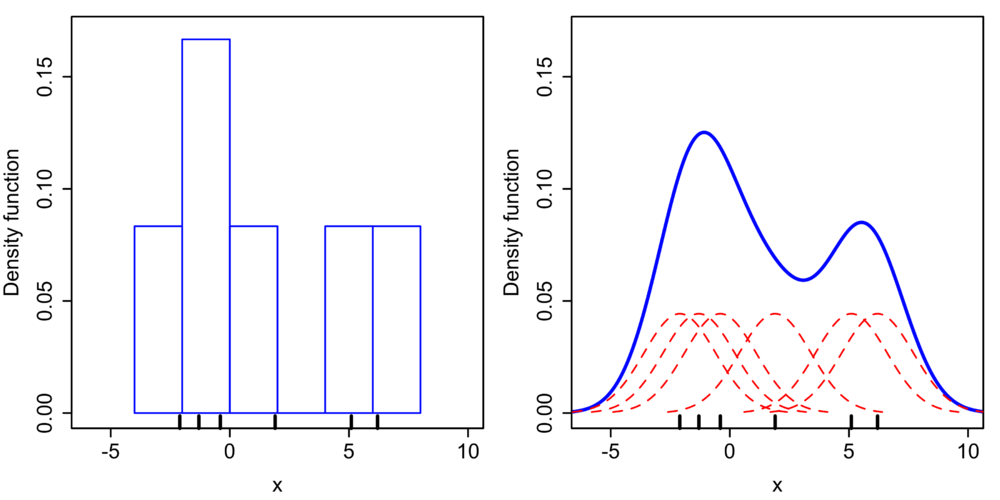
\includegraphics[width=0.618\textwidth]{images/Comparison_of_1D_histogram_and_KDE.png}
        \caption{左:直方图,右:核密度估计}
    \end{figure}


\end{frame}